\section{Aus der normalen Vorlesung}
$\mathbb{Q},\mathbb{R}$ und $\mathbb{C}$ sind Körper\\
%
%
%
\subsubsection{Definition:}
$K$ ist Körper (engl. field), wenn $0,1 \in \mathbb{K}$ verschieden und "` + "', "` $\cdot$ "', sodass für alle $a,b,c \in \mathbb{K}$ folgendes gilt.
\begin{multicols}{2} 
\begin{enumerate}
	\item $(a+b)+c = a+(b+c)$
	\item $a+b = b+a$
	\item $a+0=a$
	\item $\forall a \in \mathbb{K} \exists -a: a+(-a)=0$
	\item $(a\cdot b)\cdot c = a\cdot (b \cdot c)$
	\item $a\cdot b = b \cdot a$
	\item $a\cdot 1 = a $
	\item $a \cdot a^{-1}=1$ sofern $a\neq 0$
	\item $a\cdot (b+c)=a\cdot b + a \cdot c$
\end{enumerate}
\end{multicols}
%
%
%
\subsubsection{Beispiel:}
$\mathbb{Q}\subseteq\mathbb{R}\subseteq\mathbb{C}$\\
$\mathbb{K}=\{-1,0,1\} \qquad \mathbb{K}=\mathbb{F}_{3}$ ist ein endlicher Körper\\
\begin{tabular}{lll}
	\begin{tabular}{c|ccc}
	+ & 1 & 0 & -1\\\hline
	1 & -1 & 1 & 0 \\
	0 & 1 & 0 & -1 \\
	-1 & 0 & -1 & 1 \\
	\end{tabular}
& &
	\begin{tabular}{c|ccc}
	$\cdot$ & 0 & 1 & -1 \\\hline
	0 & 0 & 0 & 0 \\
	1 & 0 & 1 & -1 \\
	-1 & 0 & -1 & 1\\
	\end{tabular}
\end{tabular}
%
%
%
\subsubsection{Schreibweise:}
$ a+(-b) = a-b \qquad a\cdot b^{-1} = \frac{a}{b}$
%
%
%
\subsubsection{Behauptung:}
$b+c = c \mathop{\Rightarrow}\limits^{!} b = 0$\\
DENN: $b=b+(c+(-c))=(b+c)+(-c)=c+(-c)=0$\\
Insgesamt folgt $0 \cdot a = 0$  \\
%
%
%
\subsubsection{ }
$\mathbb{R} = \mathbb{C} \ni z = a+bi \qquad a,b \in \mathbb{R}$
\begin{figure}[H]
\centering
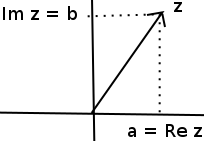
\includegraphics[width=0.2\textwidth]{mainmatter/chapter3/pics/gauszschezahlenebene.png}
\caption{Die Gaußsche Zahlenebene}
\end{figure}
$\vert z \vert = \sqrt{a^{2}+b^{2}}$ \qquad Arg$z=\measuredangle (1,z)$\\
 "` + "' komponentenweise "` $\cdot$ "' $(a+bi)(c+di)=(ac+db)+i(bc+ad)$\\
%
%
%
\subsubsection{neutrales Elements der Multiplikation}
$z=a+bi$\\
$\overline{z}=a-bi$
$z\overline{z}=a^{2}+b^{2} \in  \mathbb{R}$
$\Rightarrow z\cdot \frac{\overline{z}}{\vert z \vert^{2}} = 1$
%
%
%
\subsubsection{Addition:}
\begin{figure}[H]
\centering
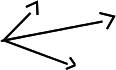
\includegraphics[width=0.1\textwidth]{mainmatter/chapter3/pics/addition.png}
\caption{Addition zweier Vektoren}
\end{figure}
%
%
%
\subsubsection{Multiplikation:}
\begin{figure}[H]
\centering
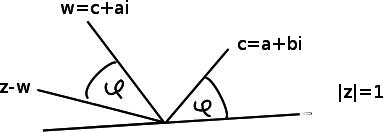
\includegraphics[width=0.3\textwidth]{mainmatter/chapter3/pics/multiplikation.png}
\caption{Multiplikation zweier Vektoren}
\end{figure}
$\begin{pmatrix} c \\ d \end{pmatrix}\begin{pmatrix}a \\ b \end{pmatrix} \rightarrow \begin{pmatrix}a & -b \\ b & a \end{pmatrix}\begin{pmatrix}c \\ d\end{pmatrix}$
%
%
%
\subsubsection{Satz:}
Bei der Multiplikation komplexer Zahlen werden die Beträge multipliziert und die Winkel addiert.
%
%
%
\subsubsection{Korollar (de Moivre)}
$(\cos\varphi + i\sin\varphi)^{n}=\cos(n\varphi)+i\sin(n\varphi)$
%
%
%
\subsubsection{Definition:}
Ein Polynom in $z$ mit Koeffizienten in $K$ ist ein Ausdruck der Form $a_{n}z^{n}+a_{n-1}z^{n-1}+\dotsc +a_{1}z+a_{0} \qquad a \in \mathbb{K}$
%
%
%
\subsubsection{Beispiel:}
$z^{n}=a$
%
%
% 
\subsubsection{Satz:}
$a\in \mathbb{C}:$ Die Gleichung $z^{n}=a$ hat genau $n$ Lösungen in $\mathbb{C}$.\\
$n=2 \qquad a=\alpha+i\beta \qquad \gamma=\sqrt{\alpha^{2} + \beta^{2}} \qquad z^{2}=a$
%
%
%
\subsubsection{Winkelhalbierende:}
$z_{1,2}=\pm(\sqrt{\frac{\gamma + \alpha}{2}} + \sqrt{\frac{\gamma-\alpha}{2}}i)$\\
$z_{1}^{2}=\frac{\gamma+\alpha}{2}-\frac{\gamma-\alpha}{2}+i\sqrt{\frac{\gamma^{2}-\alpha^{2}}{4}}=\alpha+i\beta=a$\\
$x^{2}+px+q=(a+\frac{p}{2}-(\frac{p^{2}}{4}-q)=(x+\frac{p}{2}+\sqrt{\frac{p^{2}}{4}-q})(x+\frac{p}{2}-\sqrt{\frac{p^{2}}{4}-q})$\\
$\frac{p^ {2}}{4}-q>0$ (Dies ist nur so in den reellen Zahlen)
%
%
%
\subsubsection{Satz:}
$p,q\in\mathbb{C}.$ Dann gibt es $\alpha,\beta\in\mathbb{C}.$ $x^{2}+pxüq=(x-\alpha)(x-\beta)$ kubische Gleichung hierauf zurück führbar.\\
$x^{3}=px+q\Rightarrow x=a+\frac{p}{3u} \qquad u=\sqrt[3]{\frac{q}{2}+\sqrt{(\frac{q}{2})^{2}-(\frac{p}{3})^{3}}}$\\
$\mathbb{N}\subset \mathbb{Z}\subset\mathbb{Q}\subset\mathbb{R}\subset\mathbb{C}$ ("`erstmal zuende"'-polynome lösbar)